\chapter{The thermal conductivity of strained graphene \label{chap:therm}}
The atypical thermal conductivity of graphene has been attributed to the out of plane acoustic (ZA) phonons.
These phonons are believed to contribute in two ways that conflict so much that if the ZA phonons were a person, they might be characterized as productive egomaniacs.
On one hand, they are believed to productively enable graphene's very high thermal conductivity by contributing more than 70\% of the thermal conductivity of suspended graphene \cite{Lindsay2010}.
On the other hand, they are thought to suppress the potentially divergent thermal conductivity contributions from the in-plane acoustic phonons \cite{Pereira2013,Bonini2012}.
Both of these opposing contributions are linked to the abnormal quadratic dispersion of the ZA phonons.
Currently, the theoretical understanding of this interesting and unique system is based solely on the observation that the thermal conductivity of supported graphene is smaller than suspended graphene \cite{Lindsay2010}.
Here we further test the theoretical understanding by measuring how the thermal conductivity is altered when strain and pressure modify the ZA phonons.
We observe no absolute indications that either strain or pressure affect the thermal transport in the atypical ways which might be expected for ZA phonon dominated transport.
This information should help us understand the importance of the ZA phonons and further test our understanding of graphene's high thermal conductivity.

We begin be describing past experimental measurements of graphene's thermal conducting with emphasis on the diminished thermal conductivity of supported graphene.
Next, we review the theoretical explanation of this observation and summarize the predicted effect of strain.
Finally, we discuss our experimental measurements starting with a description of the measurement, followed by an explanation of the data analysis, and finishing with a discussion of our results.

\section{Experimental background \label{sec:therm:Exp}}
In the first measurements of graphene's thermal conductivity, Balandin and coworkers reported a record high thermal conductivity of roughly 5000 W/m-K \cite{Balandin2008} in suspended graphene.
Shortly thereafter measurements of supported graphene showed a more modest thermal conductivity of roughly one sixth of the original value \cite{Seol2010}.
This discrepancy has been the source of several studies in the years since.

The original measurements were performed on suspended graphene samples using an optical technique.
This creative technique uses a laser excitation to heat the sample and the temperature induced energy shift of the Raman scattered light to measure temperature.
The laser excitation provides both a heat source and a thermometer.
When used in conjunction with a heat transfer model, this is enough to determine the thermal conductivity.
This technique has advantages and disadvantages.
The required samples are very simple to fabricate and the measurement is fairly standard.
However, the measured thermal conductivity depends on a variety of hard to measure parameters including the optical absorption of the graphene, the laser spot size, and the temperature dependence of the phonon modes.
What's more, the results depend on the accuracy of diffusive thermal transport models which cannot account for ballistic transport phenomena.

The simplicity of the optical technique has spurred its use in studying aspects of thermal transport in suspended FLG and the Raman measurement technique has since been advanced in a series of publications \cite{Balandin2008,Faugeras2010,Cai2010,Ghosh2010,Lee2011,Chen2011a,Chen2012}.
Faugeras \textit{et al.} showed that the symmetry of graphene over a circular microchamber simplifies the heat transfer model.
Additionally, they validated the use of phonon energy shifts as a temperature measurement by using the Raman Stokes to anti-Stokes ratio as an independent measurement \cite{Faugeras2010}.
Cai \textit{et al.} advanced the thermal transport model by including the heat transfer to the substrate instead of treating the edge of the microchamber as a heat sync.
Chen \textit{et al.} included thermal conductivity to the surrounding gas but not the substrate \cite{Chen2011a}.
As described in Appendix \ref{chap:HTM}, the thermal model used to interpret our results combines the models in these works.

The more modest value for the thermal conductivity of supported graphene was measured with a different technique \cite{Seol2010}.
The measurement was direct; it used resistive heaters to create temperature gradients and solid state thermometers to measure the temperature.
The thermal conductivity was then determined directly from the thermal resistance of the graphene.
Although this technique has less error sources, the measurements and sample fabrication are much more difficult.
As a result, there has been only one other measurement of the thermal conductivity of graphene using this technique \cite{Jang2010}.

Figure \ref{fig:therm:lit} summarizes all of the reported room temperature thermal conductivity measurements of single layer graphene.
It is clear that graphene's thermal conductivity is negatively effected by the presence of a supporting or encasing bulk material.
The thermal conductivity decrease from a value of roughly 2000 W/m-K for suspended graphene, to a value close to 500 W/m-K for graphene supported on one side, to a value of less than 160 W/m-K for graphene encased in SiO$_2$ \cite{Jang2010}.
The different thermal conductivities cannot be attributed to the different measurement techniques.
A nanoscale thermal conductivity measurement also observed suppressed thermal conductivity in supported FLG \cite{Pumarol2012}.
The observation of suppressed conductivity has driven the theoretical work described in the next section.

\begin{figure}
	\begin{center}
	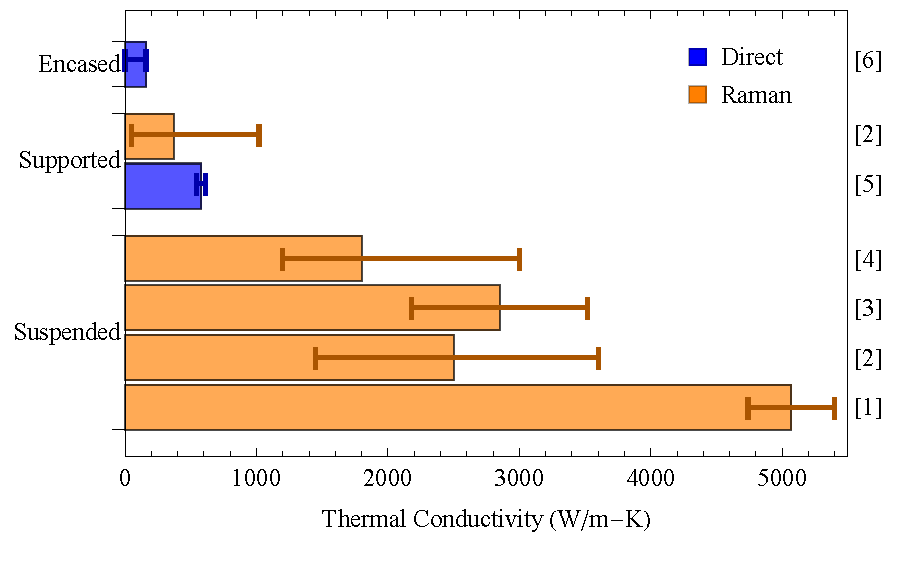
\includegraphics{Figs_Thermal/Thermal_lit.pdf}
	\end{center}
	\caption[Environmental dependence of graphene's thermal conductivity]{
	\label{fig:therm:lit}
		Summary of the reported values of the room temperature thermal conductivity of monolayer graphene grouped by the environment of the graphene: Suspended, supported on a bulk substrate, and encased in amorphous SiO$_2$.
		The color code indicates whether the measurements were performed using the Raman technique or a direct technique.
		The numbers on the right indicate the source: [1] is \cite{Balandin2008}, [2] is \cite{Cai2010}, [3] is \cite{Chen2011a}, [4] is \cite{Lee2011}, [5] is \cite{Seol2010}, [6] is \cite{Jang2010}.
		Error bars are taken from the literature.
	}
\end{figure}

\section{Theoretical background}
Lindsay and coworkers argue that ZA phonon dominated thermal conductivity in suspended graphene explains the observed environmental dependence of the thermal conductivity.
They argue that the large, 70 \%, contribution of the ZA phonons comes about for two reasons.
First, the quadratic dispersion of the ZA phonons gives them a higher density of states throughout the BZ than linearly dispered in-plane phonons.
Second, the in-plane reflection symmetry provides a selection rule that limits the scattering phase space \cite{Lindsay2010}.
ZA phonon dominated thermal transport is consistent with the observed suppression of the thermal conductivity in supported graphene.
When the graphene is in contact with bulk materials the ZA phonons either leak into the surrounding media, are scattered by it, or are dampened by it thereby lowering the thermal conductivity.
The quadratic nature of the ZA phonons should not only be a feature of monolayer graphene, but should persist for FLG as well \cite{Lindsay2011}.

The ZA phonons are also believed to limit the potentially divergent thermal conductivity contribution of the in-plane phonons.
Klemens showed that the linear in-plane acoustic phonons should contribute a logarithmically divergent thermal conductivity in graphene \cite{Klemens2001}.
This divergence follows from the frequency dependence of the terms which make up the thermal conductivity, $\kappa=\frac{1}{3} \int C v_G l(\omega) \rho(\omega) \ d\omega $, where $\kappa$ is the thermal conductivity, $C$ is the specific heat, $v_G$ is the group velocity of the acoustic phonons, $l(\omega)$ is the scattering length, and $\rho(\omega)$ is the density of states.
For a two dimensional phonon gas with linear dispersion, $\rho(\omega) \propto \omega$; while for anharmonic scattering between linear acoustic phonons, $l(\omega) \propto 1/\omega^2$.
Hence, in the absence of extrinsic scatterers the integrand scales as $1/\omega$ and $\kappa$ diverges logarithmically.
The logarithmic divergence in $\omega$ should translate to a logarithmic divergence in device size \cite{Klemens2001}.
Larger devices should exhibit larger thermal conductivities because they support more of the long wavelength phonons that contribute strongly to the thermal conductivity.
To date this logarithmic divergence has not been observed \cite{Chen2011a}.

Pereira and coworkers believe that the ZA phonons suppress this divergence.
When these ZA phonons are neglected in equilibrium molecular dynamics simulations, the thermal conductivity diverges in agreement with Klemens; when they are included, the thermal conductivity converges to a large, but finite value \cite{Pereira2013}.
It is believed that this is due to the ZA phonons near the center of the BZ.
With near zero group velocity these phonons cannot enhance thermal conductivity, but, with a large population they can effectively scatter the in-plane phonons and eliminate the divergence.
Thus, the ZA phonons are the main contributor to graphene's thermal conductivity only because the low energy ZA phonons suppress the divergent thermal conductivity of the in-plane phonons.

Simulations by both Pereira \cite{Pereira2013} and coworkers and Bonini and coworkers \cite{Bonini2012} show that strain could act to liberate the divergent thermal conductivity contribution of the in-plane phonons.
By linearizing the ZA phonon modes near the $\Gamma$ point, strain decreases the density of states of the zero group velocity ZA phonons and limits the scattering of the in-plane phonons.
Uniaxial strain of 2 \% should reduce this scattering enough to realize the divergent thermal conductivity of the in-plane phonons \cite{Pereira2013} while for biaxial strain any amount of strain should be enough \cite{Bonini2012}.

\section{Tuning the ZA phonon}
Although the theory discussed to this point is convincing, it deserves further testing.
It was built around only two data points: The high thermal conductivity of suspended graphene and the lower thermal conductivity of supported graphene.
Further, the resulting theory relies on the exotic, quadratically dispersed, ZA phonons which have only been measured directly in graphene mechanical resonators.
Here we take advantage of the two dimensional nature of graphene which enables additional ways to study the thermal transport.

The ZA phonons can be continuously tuned while the thermal conductivity is measured \textit{in situ} using the device geometry from Chapter \ref{chap:fri}.
The phonons are altered in two ways.
First, the strain induced in pressurized graphene sealed microchambers linearizes the ZA phonon dispersion.
As discussed in the previous section, this might increase the thermal conductivity by liberating the divergent thermal conductivity of the in-plane phonons \cite{Pereira2013,Bonini2012}.
Second, the gas surrounding the suspended graphene should lower the lifetime of the ZA phonons.
This has been observed in graphene mechanical resonators which exhibit decreased quality factors in ambient pressure compared to vacuum \cite{Bunch2007}.
Lowering the phonon lifetime should lower their contribution to the thermal conductivity.
In this section we describe our efforts to provide deeper insight into the mechanism behind the high thermal conductivity of suspended graphene by measuring the effect of strain and pressure on thermal conductivity.

\subsection{Thermal measurements}
The experimental geometry described in Section \ref{sec:fri:Exp} not only enables the ZA phonons to be tuned, it allows allows the effects of strain and pressure to be decoupled.
The phonons are tuned by setting the external pressure, $P$, to gauge pressures which range from -0.1 MPa of vacuum to 0.69 MPa of overpressure using argon as a pressure transfer medium.
Measuring with the external pressure both greater than and less than the pressure inside the microchamber, $P_0$, isolates strain and pressure effects.
Pressure effects should increase monotonically with pressure while strain effects should come to a minimum when $P=P_0$ and the graphene is flattened out.
Thus, the symmetry of the observed trends about $P_0$ allows pressure and strain effects to be decoupled.

The Raman technique described in Section \ref{sec:therm:Exp} is used to measure the thermal conductivity.
Linearly polarized, 514.5 nm laser light from an argon ion laser is focused on the center of the microchamber.
The focused beam waist, measured the same way as was done in Section \ref{sec:fri:Raman}, is $0.66 \pm 0.04$ nm.
The power which reaches the sample is tuned by changing the laser power, not by changing ND filters.
This ensures that the centering of the beam is not power dependent.
The power which reaches the sample is calculated from the power measured at the exit port of the Renishaw by using the system throughput of $0.67 \pm 0.01$.
The laser stability over the measurement period is 2 \%.
Raman spectra measured at several incident powers can be used to measure the temperature by monitoring the energy of the measured phonon modes.

The temperature is measured using the heating induced shifts of the G and 2D energies: $\Delta \omega=\chi \Delta T$, where $\Delta T$ is the change in temperature and $\chi$ represents the temperature dependence arising due to anharmonicities \cite{Bonini2007}.
As starting points we use the values measured by Chen \textit{et al.} on suspended CVD graphene: $\chi_G=-(4.4 \pm 0.3) \times 10^{-2} \ cm^{-1}/K$, $\chi_{2D}=-(7.2 \pm 0.2) \times 10^{-2} \ cm^{-1}/K$ \cite{Chen2011a}.
Other measurements report lower values of $\chi_G$ and $\chi_{2D}$ \cite{Calizo2007}, and hence, higher thermal conductivities \cite{Balandin2008}.
These values were not used because they were measured on supported graphene where the different thermal expansion coefficients of graphene and its supporting substrate could be more of an issue.
In addition to the temperature induced energy shifts, the phonon modes are also influenced by strain, which can cause order of magnitude larger shifts.
To isolate the temperature induced energy shift, at each applied pressure two spectra are measured: One at a lower power, $P_{lo}$, and one at a higher power, $P_{hi}$.
Both measurements have a common strain-induced energy shift which does not influence the energy difference measured between the two powers.
The measure temperature, $T_M$, is related to the energy shift, $\Delta \omega$, by assuming a constant thermal resistance, $R=\frac{\Delta T}{P}$ where P is the absorbed power.
The measured temperature is
\begin{equation}
	T_M=T_{hi}-T_0=\frac{\Delta \omega}{\chi} \frac{P_{hi}}{P_{hi}-P_{lo}} \ , \label{eq:therm:TM}
\end{equation}
where $T_0$ is ambient temperature.
The corresponding measured thermal resistance is $R_M=T_M/P_{hi}$.
The measured values do not represent the temperature at the center of the microchamber.
They are weighted averages over the finite spot of the laser beam.

It should be noted that these temperature dependent phonon energy shifts are due to phonon anharmonicities and, as such, they may have some strain dependence.
We are ignoring this possibility here.
The Anti-Stokes to Stokes ratio could be used as an alternative, anharmonicicty independent temperature measurement.
However, we found that these measurements were not useful as they took too long and were too hard to interpret.

The heat transfer model described in Appendix \ref{chap:HTM} is used to extract the thermal parameters from the measured temperatures.
The model depends on the thermal conductivities of the suspended graphene, $\kappa_{SS}$, and the supported graphene, $\kappa_{SP}=(579 \pm 34)$ W/m-K \cite{Seol2010}, as well as the interface thermal conductivities to the gas, $g_G$, and to the substrate $g_S=(50 \pm 13) \ MW/m^2$-K \cite{Mak2010}.
An example temperature distribution predicted by this model is shown in Figure \ref{fig:therm:HTPlot}.
As one might expect, the temperature rise is the greatest in the center of the microchamber where the laser is positioned.
At the edge of the microchamber the slope is discontinuous due to the change in thermal conductivity.
Where the thermal conductivity is lower it takes a larger temperature gradient to conduct the same heat energy.
The green shaded region represents the radial envelope of the excitation profile.
It illustrates that $T_M$ is not the temperature rise at the center of the hole but is rather an average over a radial window.
Appendix \ref{chap:HTM} describes how $T_M$ can be used to find the thermal parameters.

\begin{figure}
	\begin{center}
	\begin{tikzpicture}[scale=1]

	%The temperature profile
	\node at (0,0) {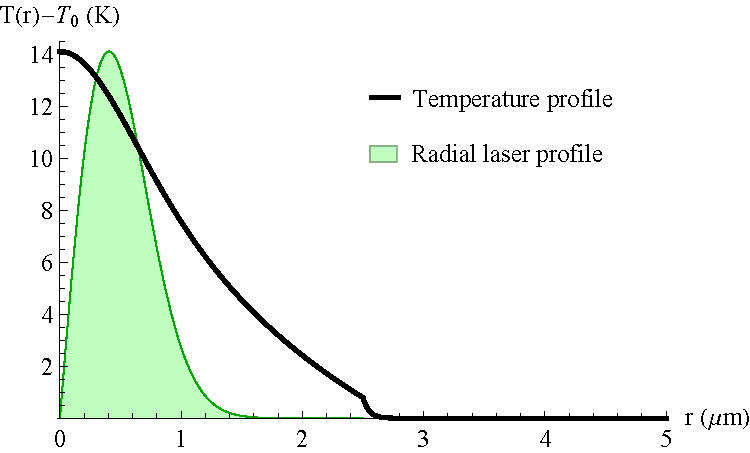
\includegraphics{Figs_Thermal/TemperatureProfile.pdf}};
	
	%The Differential Equations
	\node at (-2.8,-2.25) [fill=white, opacity=.75, text opacity=1,rounded corners=6 pt,inner sep=1.5 pt] {$\kappa_{SS} \nabla^2 T(r) + \dot{Q_L} - \dot{Q_g} =0$};
	\node at (3,-2.25) {$\kappa_{SP} \nabla^2 T(r) - \dot{Q_S} - \dot{Q_g} =0$};
\end{tikzpicture}
	\end{center}
	\caption[Expected temperature distribution in a graphene sealed microchamber heated by a centered laser]
	{\label{fig:therm:HTPlot}
		Theoretical temperature distribution in a graphene sealed microchamber heated by a centered laser.
		The black curve shows the temperature increase for a 5 $\mu$m diameter microchamber assuming that $\kappa_{SS}=2000$ W/m-K and  $g_{G}=0.03 \ MW/m^2$-K \cite{Chen2011a}.
		The radial profile of the 1.5 mW laser heat source with a 0.66 $\mu$m waist is overlaid in green.
	}
\end{figure}

The samples described in Table \ref{tab:therm:samples} were measured by taking Raman spectra with multiple excitation powers across a range of pressures.
The number of layers was found using Raman spectroscopy and optical interference, the radius and hole depths were measured using low force contact mode AFM, and the maximum strain was calculated using Hencky's model \cite{Hencky1915}.
Device fabrication was either done using the standard mechanical exfoliation technique or by using a polymer based aligned transfer technique \cite{Goossens2013T}.
Pressures were decreased in increments from 0.69 MPa to -0.1 MPa and then increased back to 0.69 in inter-spaced increments to monitor for any hysteretic response.
These measurements allowed for the extraction of the pressure dependent measured thermal resistance.

\begin{table}
	\begin{center}
	\begin{tabular}{l c c c c c c}
		\hline
		\hline
		Samples & NL 	& Radius 					& Depth 		& $\epsilon_{max}$ & Fabrication 		& Sealed? \\
		\hline
		FFF		& 1 	& $(3.09 \pm 0.04)$ $\mu$m 	& $>$ 5 $\mu$m 	& N/A	& Transferred 	 	& no \\
		SB07-1	& 1 	& $(2.74 \pm 0.08)$ $\mu$m 	& $\simeq$ 230 nm & 1.1 \%	& Exfoliated 		& yes \\
		SB08-2	& 2 	& $(1.52 \pm 0.07)$ $\mu$m 	& $>$ 3 $\mu$m 	& 0.46 \%	& Exfoliated 		& yes \\
		SB03-2	& 3 	& $(4.99 \pm 0.01)$ $\mu$m 	& $>$ 5 $\mu$m 	& 0.77 \%	& Exfoliated 		& yes \\
		\hline
		\hline
	\end{tabular}
	\end{center}
	\caption[Samples used in thermal conductivity measurements]{\label{tab:therm:samples} 
	Details of the samples used in thermal conductivity measurements. NL refers to the number of layers and $\epsilon_{max}$ is the maximum strain.}
\end{table}

\subsection{Data analysis}
This section details the analysis done to determine the measured thermal resistances from the Raman spectra.

Peak positions were found by fitting the measured spectra to representative spectral shapes.
The G peak was fit to a single Lorentzian for all four samples.
Fitting the 2D peak was more complicated because the peak shape depends on the number of layers.
For suspended monolayer graphene the 2D peak is best fit by two Lorentzians with equal widths separated by 14 wavenumbers \cite{Berciaud2013}.
To limit the number of fitting parameters, the ratio of the peak amplitudes was taken as 3.44, the average of less restricted best fits.
For bilayer graphene the 2D peak is best fit by 4 Lorentzians with equal widths \cite{Ferrari2006,Malard2007}.
The fitting parameters were restricted to an amplitude, a width, and a position by setting the separation between peaks and the relative amplitudes between peaks based on the average of less restricted best fits.
An example of the best fit to a bilayer spectra is shown in Figure \ref{fig:therm:spec} showing good agreement between the spectra measured at 0.69 MPa and the fitting function.
Since there is no well-excepted form for the trilayer 2D band, the temperatures were only determined from the G band data for sample SB03-2.
The extracted peak positions were used to analyze the response of the system to pressure and heating.

\begin{figure}
	\begin{center}
	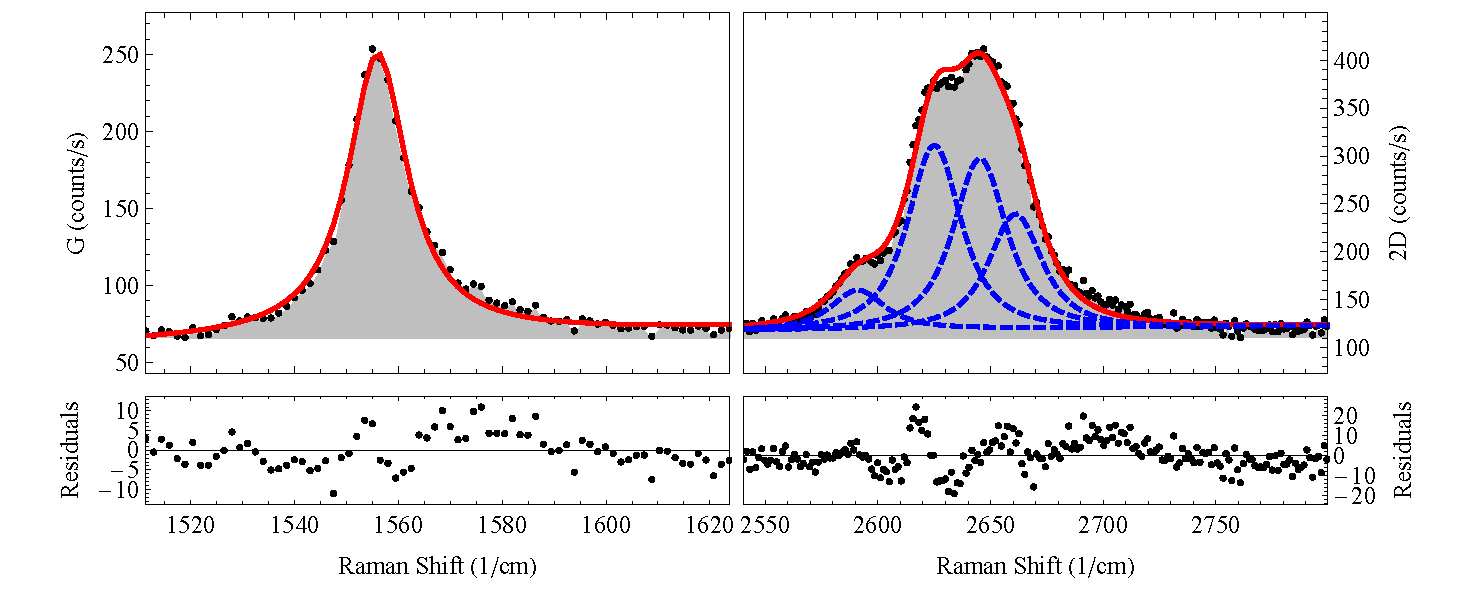
\includegraphics[scale=0.6]{Figs_Thermal/0_3mW.pdf}
	\end{center}
	\caption[Representative fit to Raman spectra for thermal conductivity measurements]{\label{fig:therm:spec}
		A representative fit to the Raman spectra taken at the center of bilayer sample SB08-2 using 2 mW of incident power at 0.69 MPa of gauge pressure.
		The restricted four Lorentzian fit to the 2D spectra matches the data well.
	}
\end{figure}

Figure \ref{fig:therm:PeakPressure}(a) shows the best fit positions of the G and 2D bands as a function of pressure for bilayer sample SB08-2.
As described in detail in Chapter \ref{chap:fri}, the overarching response is governed by the linear dependence of the Raman bands on strain.
The strain, in turn, scales roughly as $(P-P_0)^{2/3}$ where $P_0$ is the pressure inside the microchamber.
The data in the Figure is fit by the expected pressure dependence and the extracted value of $P_0$ is indicated by the black vertical line.
Samples SB07-1, SB08-2, and SB03-2 all exhibit this type of pressure dependent response.
For sample FFF, on the other hand, the Raman peak energies exhibit no measurable pressure dependence indicating that the membrane is leaky as shown in Figure \ref{fig:therm:PeakPressure}(b).
Thus, this sample is insensitive to strain effects.
The effects of laser heating in Figure \ref{fig:therm:PeakPressure} are hidden in the fine structure.
Spectra taken at higher laser powers exhibit systematically lower peak positions due to heating.

\begin{figure}
	\begin{center}
	\begin{tikzpicture}[scale=1]

	%The temperature profile
	\node at (0,0) {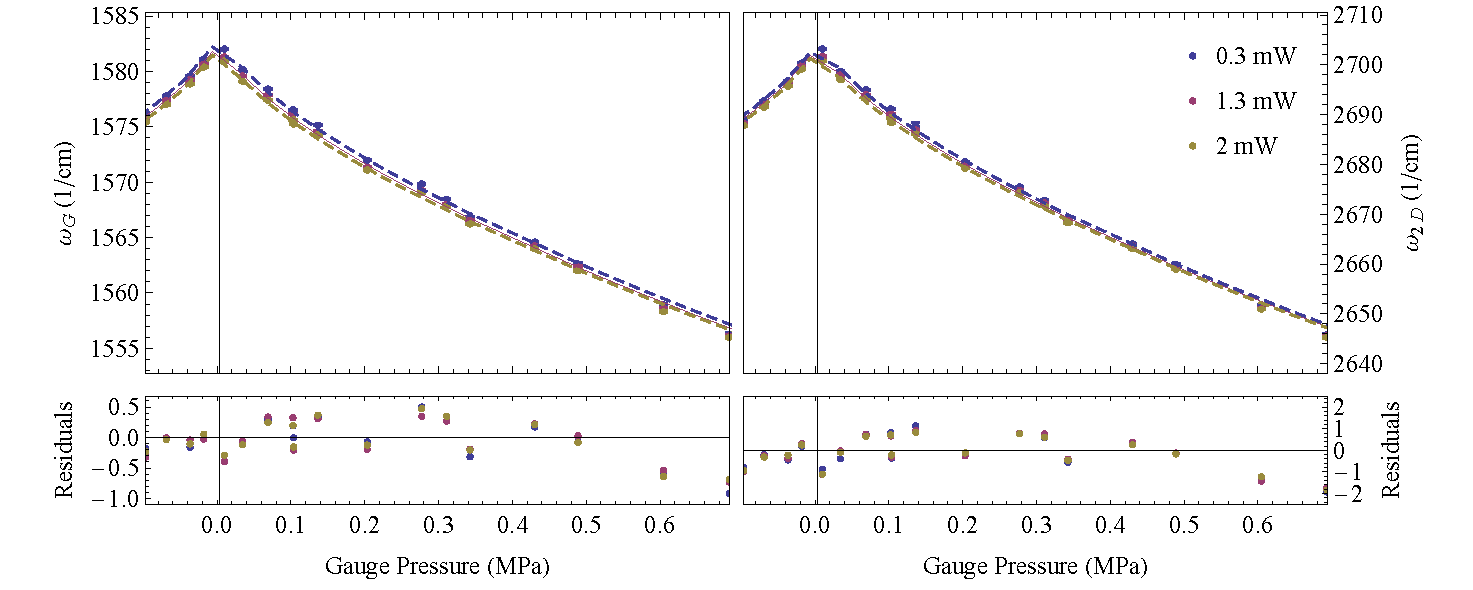
\includegraphics[scale=0.6]{Figs_Thermal/PeakPressure.pdf}};
	
	\node at (0,-6) {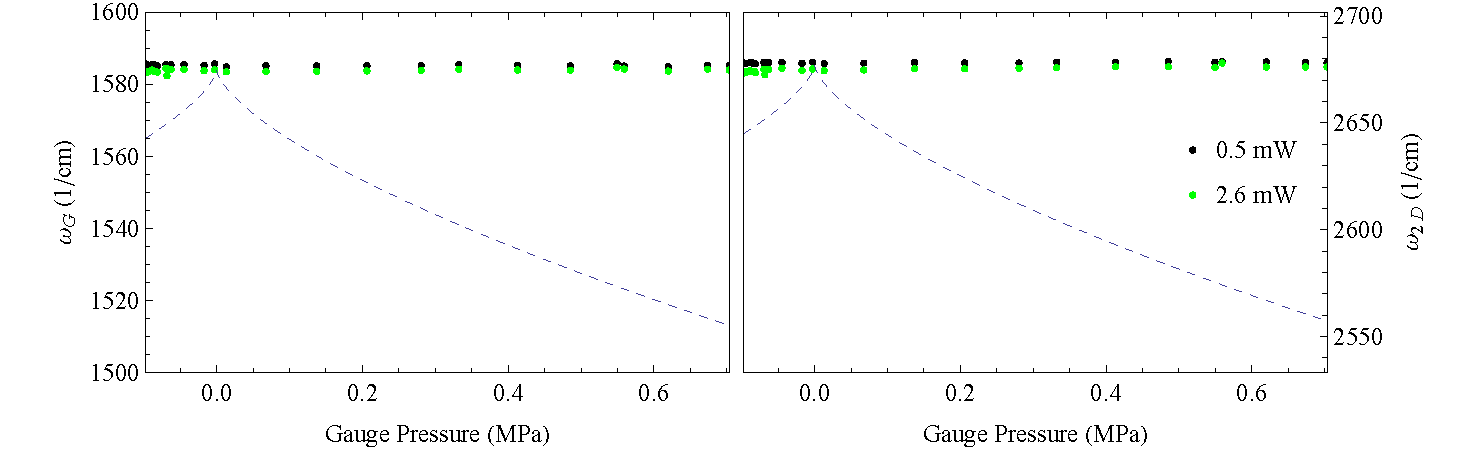
\includegraphics[scale=0.6]{Figs_Thermal/PeakPressure_FFF.pdf}};

	\node at (-7,-3.65) {\textbf{(b)}};
	\node at (-7, 3) {\textbf{(a)}};

\end{tikzpicture}
	\end{center}
	\caption[Pressure dependent peak positions]{\label{fig:therm:PeakPressure}
		The peak positions measured as a function of applied pressure with three different laser excitation powers for (a) the sealed bilayer sample SB08-2 and (b) the leaky monolayer sample FFF.
		In (a) the peak positions are fit to the expected $(P-P_0)^{2/3}$ behavior and the best fit value for $P_0$ is indicated by the black vertical line.
		In (b) the pressure response that a sealed microchamber would have undergone is indicated by the blue dashed line.
		In both cases increasing laser excitation power systematically red shifts the peak positions.
	}
\end{figure}

The use of Equation \ref{eq:therm:TM} to calculate the temperatures from the peak shifts is complicated by optical interference.
As shown in Figure \ref{fig:therm:Inter}, the measured temperatures for sample SB07-1 exhibit an oscillatory behavior in pressure that is correlated with similar oscillations in the measured G and 2D integrated areas.
This suggests that the observed behavior is driven by optical interference in the excitation beam.
As overpressure is applied to the graphene, it is pushed into the microchamber, moving it from a point where the excitation undergoes destructive interference, to a point of constructive interference, and then back to a point of destructive interference.
As the interference changes, the amount of power heating the graphene changes, and thus, so does the temperature.
The integrated areas of the G and 2D peaks also depend on the incident laser power and, thus, the correlation between the oscillations in integrated areas and the oscillations in the measured temperature is a strong indicator of optical interference effects.
The interference interpretation is further supported by the agreement between the number of interference minimum and the expected displacement at the center of the graphene.
Minimum are expected every half wavelength and from -0.1 MPa to 0.69 MPa, the graphene displaces by 508 nm or roughly one wavelength consistent with the two minimum in Figure \ref{fig:therm:Inter}.
The interference in SB07-1 is the strongest, but all of the other devices exhibit similar interference phenomena.
The Rayleigh range of the focused beam is $\sim 2.7$ $\mu$m indicating that even microchambers with depths of 8 $\mu$m might be expected to exhibit weak interference effects.
Interestingly, even leaky sample FFF shows very slight signs of interference probably due to the nonlinearity of the pressure deflection curve.
In the low pressure regime small pressure changes cause relatively large deflections which could cause interference effects; for FFF, a differential pressure of only 0.001 MPa would cause a deflection of 40 nm.
This small deflection generate a small, 0.015 \%, strain which would be challenging to detect with Raman peak shifts.
To correctly interpret the thermal response of the system, this interference must be accounted for.

\begin{figure}
	\begin{center}
	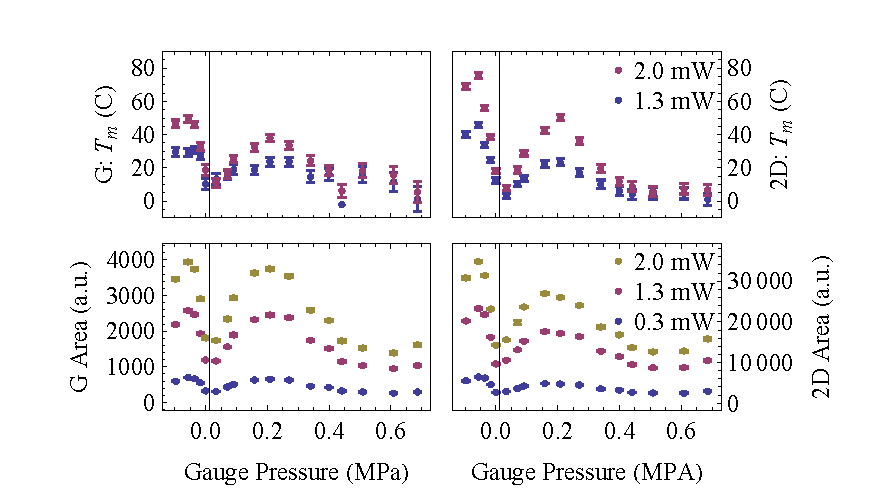
\includegraphics{Figs_Thermal/inter.pdf}
	\end{center}
	\caption[Issues with optical interference in thermal conductivity measurements]{\label{fig:therm:Inter}
		A comparison of the temperatures calculated from the shifts of the G peak (top, left) and the shifts of the 2D peak (top, right) with the measured areas of the G peak (bottom, left) and the 2D peak (bottom, right).
		Measurements were taken on monolayer sealed sample SB07-1.
		The oscillatory behavior in all four plots suggests that the observed behavior is a result of optical interference.
	}
\end{figure}

The optical interference of the excitation beam can be estimated from the oscillatory behavior of the Raman signal.
Raman interference is driven by the product of the optical interference of the incident beam and the outgoing, inelastically scattered light.
Approximating the system as a plane wave incident on a perfect mirror, the product of these two terms gives the Raman peak area as $Area=P_i 4 \sin^2(k z) \sin^2(k_R z)$ where $z$ is the distance of the graphene above the mirror, $k$ is the spatial frequency of the laser excitation, $k_R$ is the spatial frequency of the inelastically scattered light, and $P_i$ is the power of the incident beam.
The perfect mirror approximation is reasonable for silicon with light in the visible.
Using silicon's optical constants from Palik \textit{et al.} \cite{Palik1991} reproduces the approximate behavior with a negligible 2 \% constant offset.
The oscillations in the measured temperature, however, is only driven by the interference in the incident beam, $f_{int}=2 \sin^2(k z)$.
The fact that the exact depths of the microchambers are not known and that the interference is in a Gaussian beam and not a plane wave makes a direct calculation of the incident power from the oscillations in the Raman areas impractical.
Instead, we approximate the interference in the area of the Raman peak as $Area=4 P_i \sin^2(k z) \sin^2(k_R z) \simeq 4 P_i \sin^4(k z) = P_i f_{int}^2$ allowing an estimation of the interference in the excitation beam.

In addition to the interference oscillations there is a constant background underlying the G and 2D areas as shown in Figure \ref{fig:therm:Inter}.
The signal contributing to this offset is believed to be generated by light which is not interfering.
This could be a result of a rough silicon back plane or from the divergence of the beam.
Thus, the area of the Raman peak can be expressed as the sum of a not-interfering component and an interfering component with relative amplitudes $A$ and $\frac{1}{4} B$
\begin{equation*}
	Area=P_i \ A+P_i \ \frac{1}{4} B \ f_{int}^2 \rightarrow  f_{int}=2\sqrt{\frac{Area/P_i-A}{B}} \ .
\end{equation*}
$P_i A$ and $P_i (A+B)$ are then the minimum and the maximum measured integrated areas areas, respectively.
The factor of $1/4$ is included so that $B$ is the amplitude of the interference oscillation.
The intensity of the incident beam is then corrected by dividing by the normalized intensity at the sample: $(A+f_{int} \ B/4)/(A+B/8)$.
Using this correction, the thermal resistances can be calculated from the measured temperatures.
The resulting $R_M$ should be independent of interference effects up to the approximations used.

Accurate determinations of the measured thermal resistances are enabled by redundant measurements.
For samples FFF, SB07-1, and SB08-2 both the G and 2D shifts can be used to calculate $R_M$.
The values of $\chi$ reported by Chen \textit{et al.} \cite{Chen2011a} provided good agreement between G and 2D data for sample SB08-2.
However, for sample FFF, a slight offset in $\chi_G$ and $\chi_{2D}$ was required to achieve good agreement.
The values of $\chi$ for the G and 2D peaks needed to be increased and decreased by $0.6 \times 10^{-2} \ cm^{-1}/K$ respectively.
For sample SB07-1, the G and 2D measurements are presented separately.
Samples SB07-1, SB08-2, and SB03-2 were measured at three different powers providing two additional measurements of $R_M$.
Averaging all of the redundant measurements provides higher certainties.
Figure \ref{fig:therm:R_average} shows an example of the averaged $R_M$ data.
The individual $R_M$ measurements are in good agreement, justifying the averaging.

\begin{figure}
	\begin{center}
	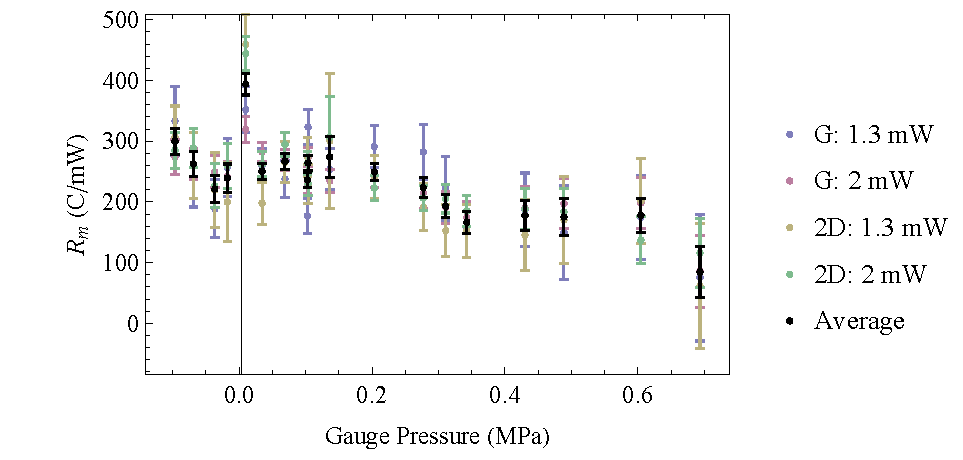
\includegraphics[scale=0.8]{Figs_Thermal/R_average.pdf}
	\end{center}
	\caption[Average pressure dependence of the measured thermal resistance]{\label{fig:therm:R_average}
		The average measured thermal resistance of bilayer sample SB08-2.
		The four different measurements used to calculate the average are in good agreement.
		The black vertical line is positioned at $P_0$.
	}
\end{figure}

In summary, the measured thermal resistance is calculated by fitting the measured spectra, using the heating shifts to determine temperatures, correcting for optical interference, and averaging over redundant measurements.
The general trends in the measurements are discussed in the following section.

\subsection{Discussion}
Figure \ref{fig:therm:Rs} shows the thermal resistance measured on the four samples.
The thermal resistance of the leaky monolayer (FFF) was roughly a factor of four larger than the sealed bilayer (SB08-2) and the sealed trilayer (SB03-2).
This is probably because the holes in the leaky monolayer decrease the thermal conductivity and increase the thermal resistance.
However, when its thermal resistance was scaled by a factor of 0.28 the pressure dependent thermal resistance of FFF agreed well with SB08-2 and SB03-2.
They all exhibit a decrease in $R_M$ with increased pressure with a dip in thermal resistance near -0.05 MPa.
The lack of symmetry about the pressure inside the microchamber ($P_0 \approx 0$) indicates that the trend is unrelated to the strain in the graphene.
This is further supported by the agreement between the sealed microchambers which are strained by pressure and the leaky microchambers which are not.
The origin of the dip at -0.05 MPa is not understood at this time.
The sealed monolayer graphene measurements, on the other hand, do display symmetry about $P_0$.
However, the correlation between these features and the optical interference in Figure \ref{fig:therm:Inter} indicates that these features could be attributed to imperfect interference corrections.
In fact, this device should be most sensitive to the approximations made in correcting the optical interference since the sealed monolayer is the most shallow and undergoes the most interference.
Thus, for monolayer graphene the observed trend is indecipherable and for bilayer and trilayer graphene in the strain regions measured (see Table \ref{tab:therm:samples}), there is no evidence for strain dependent thermal conductivity.
Additionally, no measurements show the significant decrease in $R_M$ at high pressure which would indicate the predicted strain-induced transition to divergent thermal conductivity \cite{Bonini2012,Pereira2013}.

\begin{figure}
	\begin{center}
	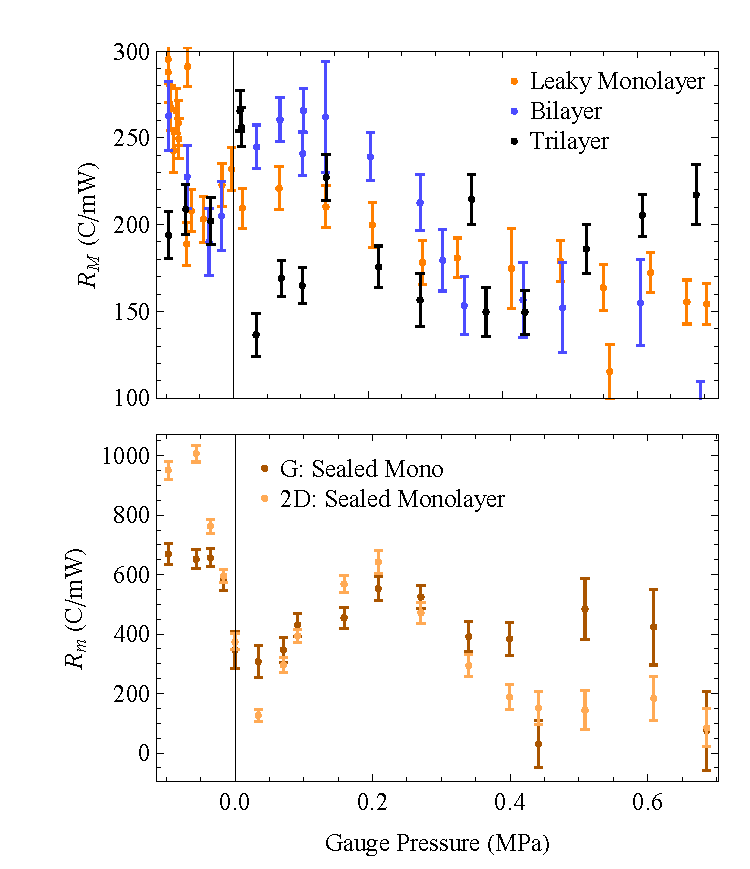
\includegraphics{Figs_Thermal/Rs.pdf}
	\end{center}
	\caption[Pressure dependent measured thermal resistances of mono-, bi-, and trilayer graphene]{\label{fig:therm:Rs}
		Comparison of the pressure dependent measured thermal resistances of sealed monolayer (SB07-1), bilayer (SB08-2), and trilayer (SB03-2) graphene as well as leaky monolayer (FFF) graphene.
		The thermal resistances of the leaky monolayer was scaled by a factor of 0.28 for easier comparison.
		Data for the sealed monolayer graphene is plotted separately to better see the trends in the data.
	}
\end{figure}

The pressure dependent measured thermal resistances seen in the leaky monolayer (FFF), the sealed bilayer (SB08-2), and the sealed trilayer (SB03-2)could originate from thermal conduction to the gas, from viscous damping of the ZA phonons, or from both.
To test if the observed behavior can be reasonably attributed only to the thermal conduction the gas, viscous damping was neglected and the interface thermal conductivity to the gas, $g_G$, was fit to the data following Appendix \ref{chap:HTM}.
Assuming that $g_G=0 \ W/m^2$-K in a vacuum, the in-plane thermal conductivity was extracted from the measurement with the largest $R_M$ measured at vacuum.
This gave $\kappa_{SS}=1070 \pm 120$ W/m-K, $\kappa_{SS}=1730 \pm 130$ W/m-K, $\kappa_{SS}= 820 \pm 40$ W/m-K for the bilayer, trilayer, and leaky monolayer samples respectively. 
One sigma confidence intervals were calculated using a Monte-Carlo technique which accounts for all known uncertainties.
The results are shown in Figure \ref{fig:therm:gs}

\begin{figure}
	\begin{center}
	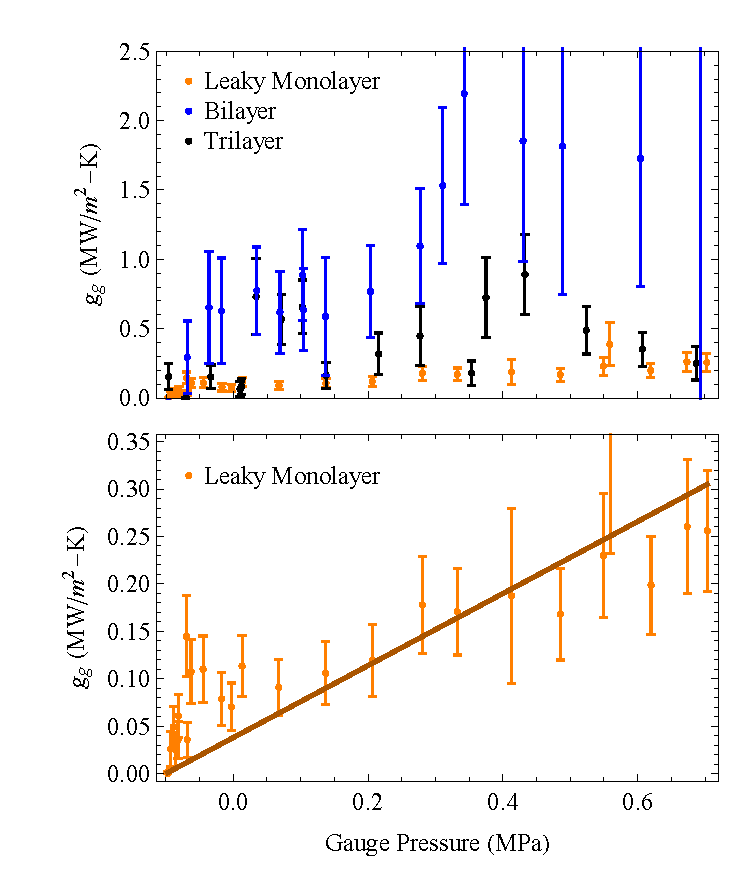
\includegraphics[scale=0.8]{Figs_Thermal/gs.pdf}
	\end{center}
	\caption[Pressure dependent interface thermal conductivity to the gas]{\label{fig:therm:gs}
		Assuming that the in-plane thermal conductivity is constant, the $R_M$ in Figure \ref{fig:therm:Rs} were used to determine the interface thermal conductivity to the gas.
		The top plot compares the values for a leaky monolayer (FFF), a sealed bilayer (SB08-2), and a sealed trilayer (SB03-2) while the bottom plot shows only the leaky monolayer data fit to a line.
	}
\end{figure}

The behavior of the interface thermal conductivity of the leaky monolayer is different than the sealed bilayer and trilayer samples.
For pressures greater than ambient pressure, the interface thermal conductivity of the leaky monolayer increases roughly linearly with pressure.
This linear trend is expected based on a kinematic model \cite{Chen2011a}.
At higher pressures there are more atoms in the gas available to conduct heat away from the sample.
Additionally, the ambient pressure value of $g_g = 0.06 \pm 0.03 \ MW/m^2$-K is in fair agreement with the previously measured value for graphene in air of $g_g = 0.029+0.051/-0.029 \ MW/m^2$-K \cite{Chen2011a}.
Thus, for positive applied pressures, the thermal response of the leaky monolayer is consistent with thermal conduction to the gas.
The thermal resistance bump near -0.1 MPa comes from the not-yet-understood dip in the thermal resistance near the same pressure.
The bilayer and trilayer samples exhibit different behavior.
Their interface thermal conductivity is higher and behaves less linearly than the leaky monolayer.
This is probably due to the gas sealed inside of these microchambers.
For low applied gas pressures, the gas in the microchamber conducts much more heat than the gas above the microchamber resulting in a fairly flat pressure response in $g_g$.
For larger pressures, the conduction to the gas above dominates the conduction to the gas below and a stronger pressure response should occur.
The flattening out of the pressure response at the highest pressures is not yet understood.

\subsection{Conclusions}
Strain and pressure dependent thermal conductivity measurements were performed on monolayer, bilayer, and trilayer graphene to gain insight into the atypical thermal conductivity in FLG.
Strain and pressure are expected to modify the quadratic ZA phonon, believed to be the main contributor to the high thermal conductivity in strained graphene.
We found that sealed bilayer and trilayer graphene devices as well as leaky monolayer graphene exhibits measured thermal resistances which decrease with pressure.
Heat conduction to the gas, viscous damping of the ZA phonons, or both effects together could cause such a trend.
In the case of the leaky monolayer, we showed that the observed thermal resistance is consistent with heat conduction to the gas.
The interpretation of the sealed bilayer and trilayer samples, however, was complicated by the gas sealed inside of the microchambers.
Measurements of leaky bilayer and leaky trilayer could eliminate this complication in the future.
Regretfully, the results for sealed monolayer graphene were indecipherable because of optical interference.
In future measurements microchambers should be fabricated much deeper to eliminate these effects.

We did not observe the predicted strain induced transition to divergent thermal conductivity \cite{Bonini2012,Pereira2013} in any of our devices.
This might be because we did not reach high enough strains, because the strain distributions which develop in graphene sealed microchambers are not suitable, or possibly because the predictions are incorrect.